%%%%%%%%%%%%%%%%%%%%%%%%%%%%%%%%%%%%%%%%%%%%
\section{Challenges and Opportunities in Engineering}

{
\paper{engineeringchallenges.org/challenges.aspx}
\begin{frame}{Challenges in Engineering}
  \begin{columns}
    \begin{column}{.6\linewidth}
    \begin{itemize}
    \item \textbf{Advance Personalised learning}
    \item \textbf{Make Solar Energy Economical}
    \item \textbf{Enhance Virtual Reality}
    \item \textbf{Reverse-engineer the brain}
    \item \textbf{Egineer better medicines}
    \item \textbf{Advance Health Informatics}
    \item \textbf{Restore and improve urban infrastructure}
    \item \textbf{Secure cyberspace}
    \item \textbf{Provide access to clean water}
    \item \textbf{Provide energy from fusion}
    \item \textbf{Develop Carbon Sequestration Methods}
    \item \textbf{Engineer the tools for science discovery}
    \end{itemize}
  \end{column}

  \begin{column}{.4\linewidth}
      \begin{figure}
        \centering
        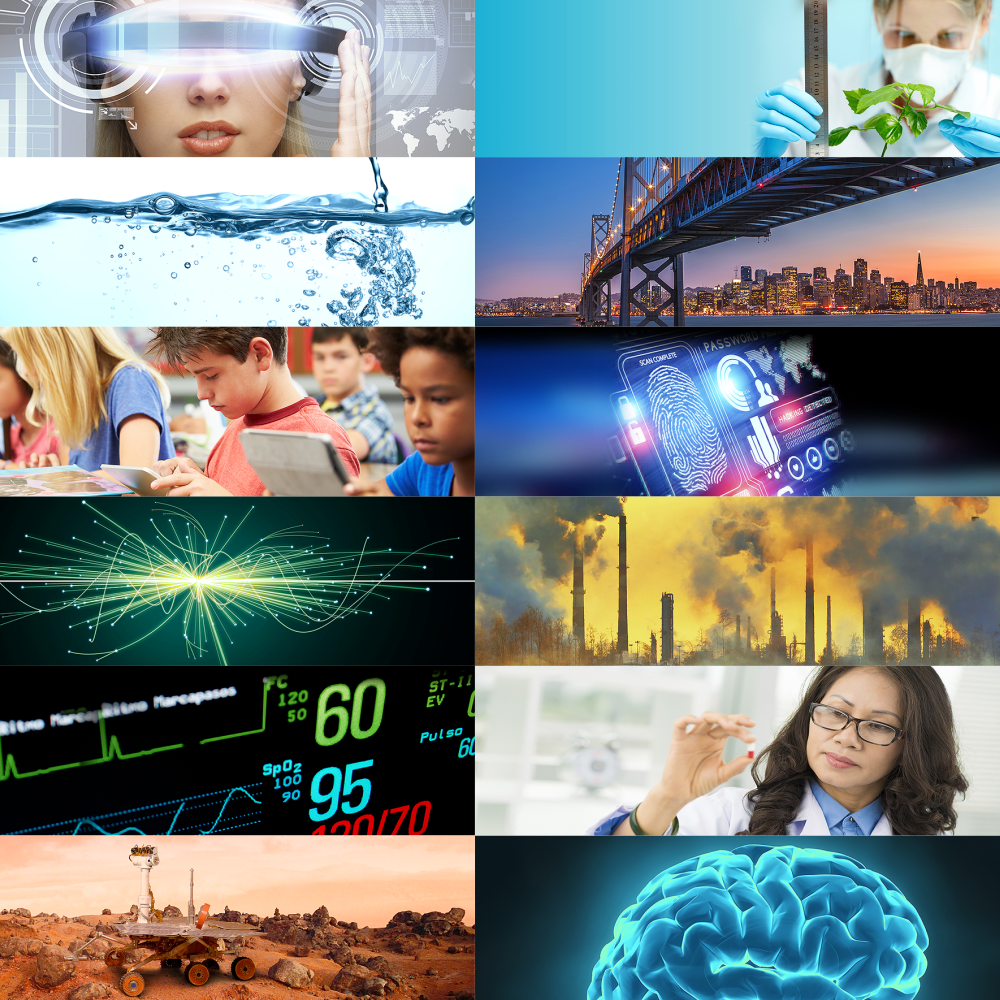
\includegraphics[scale=0.2]{./figs/challenges/versions/drawing-v01.png}
        \caption{}
      \end{figure}
    \end{column}
  \end{columns}

\end{frame}
}






%%%%%%%%%%%%%%%%%%%%%%%%%%%%%%%%%%%%%%%%%%%%
\subsection{Engineering as Multidisciplinary Field}

{
\paper{\textbf{Khanna and Kumar 2020} in Engineering 4.0: Future with Disruptive Technologies, DOI:10.1007/978-981-15-1137-07}
\begin{frame}{Engineering as Multidisciplinary Field}
    \begin{figure}
        \centering
        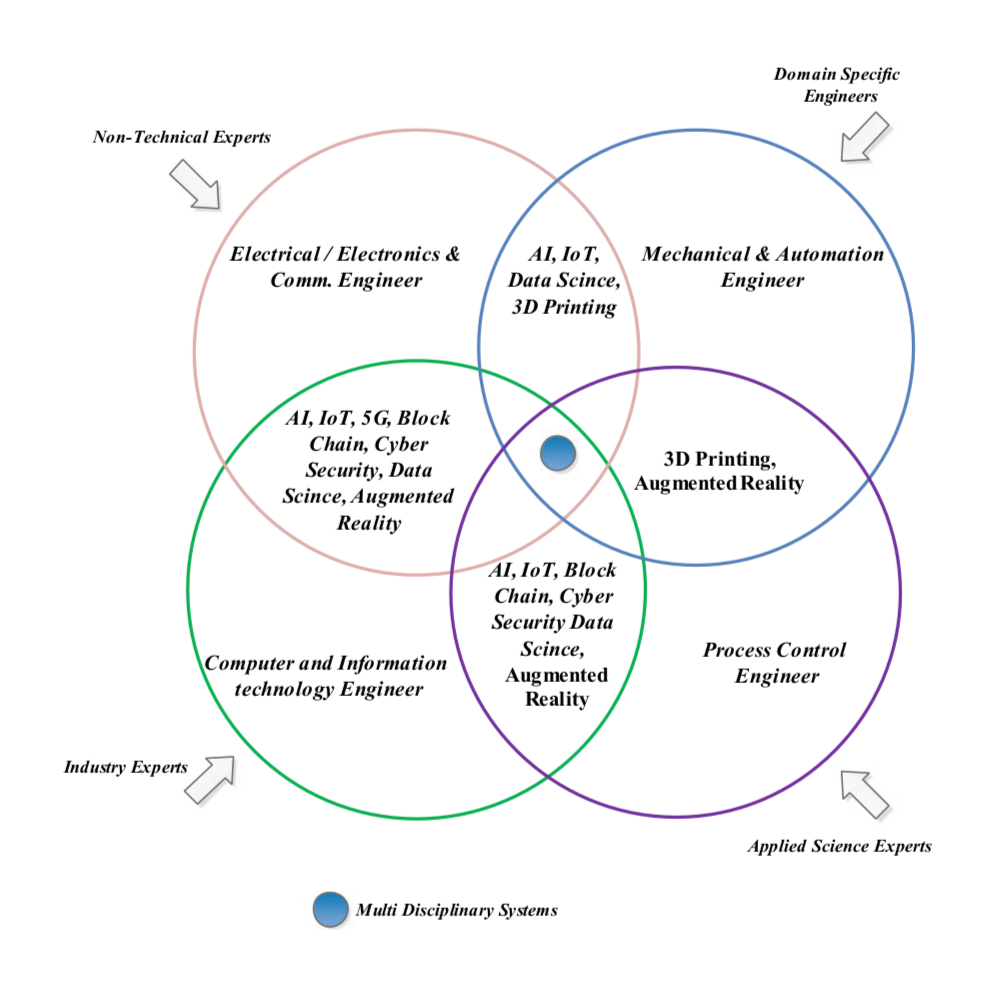
\includegraphics[width=0.55\linewidth]{./figs/multidisciplinary-engigneering/versions/drawing-v00.png}
        \caption{}
    \end{figure}
\end{frame}
}


%%%%%%%%%%%%%%%%%%%%%%%%%%%%%%%%%%%%%%%%%%%%
\subsection{Mechatronics and Robotics Engineering}
\begin{frame}{Robotics Engineering }
    \begin{figure}
        \centering
        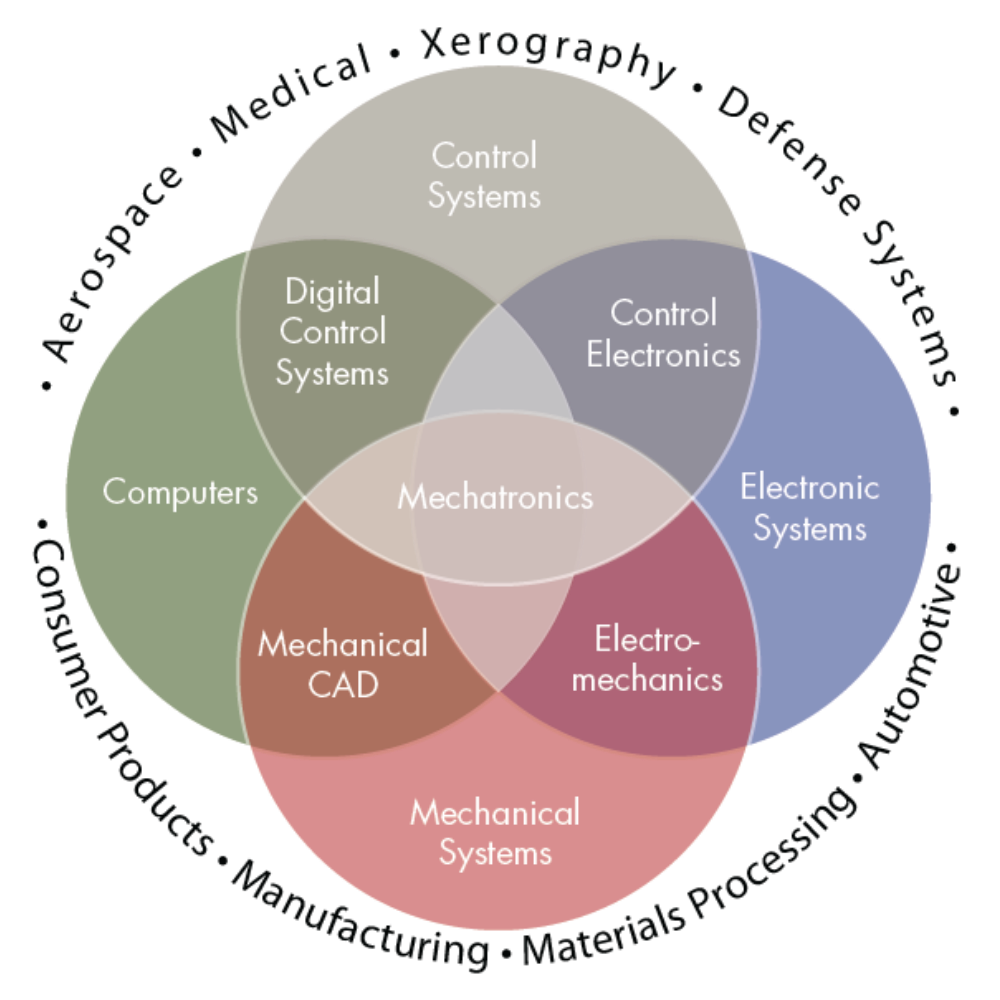
\includegraphics[width=0.5\linewidth]{./figs/robotics/versions/drawing.png}
        \caption{}
    \end{figure}
\end{frame}


%%%%%%%%%%%%%%%%%%%%%%%%%%%%%%%%%%%%%%%%%%%%
\subsection{Open-source projects}
{
%\paper{\textbf{Xochicale 2020} in Conf. of Reproducibility, Replicability and Trust in Science \faGithub github.com/mxochicale/rrts2020}
\begin{frame}{Open-source projects}
    \vspace{-00mm}
      \begin{figure}
        \centering
        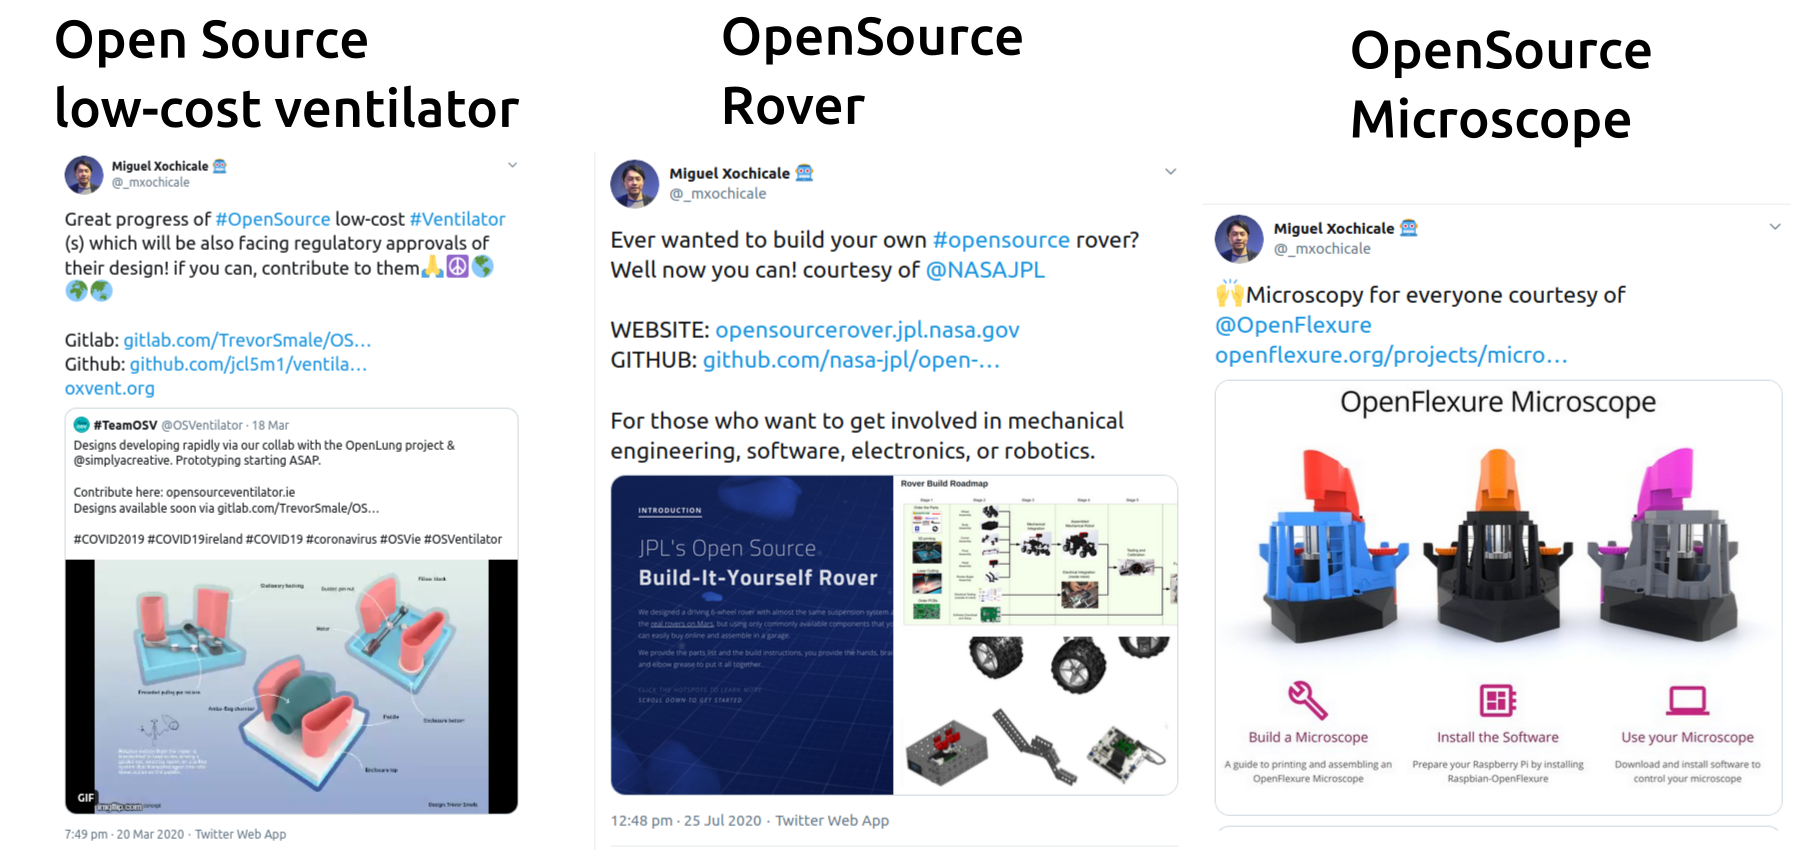
\includegraphics[width=\linewidth]{./figs/oa-projects/versions/drawing-v00.png}
        \caption{}
      \end{figure}
\end{frame}
}

